\documentclass[tikz,border=4mm]{standalone}
\usetikzlibrary{positioning,arrows.meta,calc}

\begin{document}
\begin{tikzpicture}[
  >=Latex,
  x=1cm,y=1cm,
  node/.style={draw, circle, minimum size=7mm, inner sep=0pt},
  hnode/.style={draw, rounded corners=2pt, minimum width=26mm, minimum height=7mm, align=center},
  edgelab/.style={midway, sloped, fill=white, inner sep=1pt, font=\scriptsize},
  small/.style={font=\footnotesize}
]

% --- Nodes ------------------------------------------------------
\node[node] (x) at (0,0) {$x$};

% hidden layer (6 ReLU units)
\foreach \i/\yy in {1/3, 2/2, 3/1, 4/-1, 5/-2, 6/-3}{
  \node[hnode, anchor=west] (h\i) at (2,\yy)
    {$h_{\i}(x)=\mathrm{ReLU}(w_{\i}x+b_{\i})$};
}

\node[node, right=6cm of x] (y) {$\hat{y}$};

% --- Edges: input -> hidden (label w_i) ------------------------
\foreach \i/\yy in {1/3, 2/2, 3/1, 4/-1, 5/-2, 6/-3}{
  \draw[->, thick] (x.east) -- ($(h\i.west)!0.12!(h\i.east)$)
    node[edgelab, above] {$w_{\i}$};
}

% --- Edges: hidden -> output (label v_i) -----------------------
\foreach \i in {1,...,6}{
  \draw[->, thick] (h\i.east) -- (y.west)
    node[edgelab, above] {$v_{\i}$};
}

% --- Extra annotations -----------------------------------------
\node[small, align=left, below=0.4cm of y] (eq)
  {$\displaystyle \hat{y}(x)= d + \sum_{k=1}^{6} v_k\, h_k(x)$};

\node[small, align=left, below=0.2cm of x]
  {$\text{1-hidden-layer ReLU network (graph view)}$};

% Optional: show each unit's breakpoint at x^* = -b_i/w_i
% (purely as a legend text; not drawn on axis)
\node[small, align=left, right=0.2cm of eq]
  {$x_k^{\ast}=-\dfrac{b_k}{w_k}$};

\end{tikzpicture}
\end{document}
